%This is the second chapter of the dissertation

%The following command starts your chapter. If you want different titles used in your ToC and at the top of the page throughout the chapter, you can specify those values here. Since Columbia doesn't want extra information in the headers and footers, the "Top of Page Title" value won't actually appear.

\pagestyle{cu}
\graphicspath{{./Chapter2/Figures/}}
\chapter[Liquid Xenon and Time Projection Chambers][Liquid Xenon and Time Projection Chambers]{Liquid Xenon and Time Projection Chambers}
\label{chap:liquid_xe}

Liquid xenon (LXe) direct detection experiments have dominated the sensitivity for WIMP masses $\gtrsim 20$ for approximately as
decade.  Even over liquid argon (LAr) the LXe results have been paved the way to new limits, surpassing on the way only those of other
LXe experiments.

Commercial business, such as steelmaking and coal gasification, rely relatively pure oxygen or nitrogen.  During the separation,
the small amount of xenon and krypton in the air is extracted into a mixture as a by-product.  A distillation process can uncouple
the two, leaving highly pure xenon.

%====================================
\section{General Properties}
\label{sec:properties}
Xenon has an atomic number of 54 with a mean mass of 131.293 g mol$^{-1}$.  Because it is a noble gas it does not easily undergo chemical
reactions with other elements.  It makes up 87 parts per billion (ppb) of the Earth's atmosphere at a density of
5.894 g L$^{-1}$.  \tabref{tab:xe_properties} gives some general chemical properties for xenon.

Xenon is the heaviest noble gas that is non-radioactive, with an atomic molar mass of $A = 131.293\ \mathrm{g\ mol^{-1}}$.  The naturally
occurring Xe isotopes are listed in
\tabref{tab:xe_isotopes}.  $^{136}Xe$, with a fractional percentage of 8.8573\%,
has been measured to undergo double beta decay with a half-life of $> 2.4 \times 10^{21}\ \mathrm{yrs}$ via
$2\nu \beta^{-} \beta^{-}$.  So while technically naturally occurring xenon is radioactive, the process is extremely rare.

Primary and secondary scintillation, which are the measured parameters in a time-projection chamber, occur when a particle interacts
with a Xe atom.  In the case of a neutron or neutrino scattering from the Xe nucleus a number of nuclear excitations are possible,
and are listed in \tabref{tab:xe_radioactive}.  The 39.6 and 80.2 keV lines from $^{129}$Xe and $^{131}$Xe are short-lived and typically cannot
be resolved from the scintillation of the scatter.  However, the 163.9 and 236.14 keV lines from $^{131\mathrm{m}}$Xe and
$^{129\mathrm{m}}$Xe are long-lived
enough to become uniformly distributed throughout the detector and can be used as a calibration source and measuring the electron
lifetime (\chapref{chap:purity}).

Xenon has several advantages that make it a good source for DM detection.  At \$2000 it is scaleable for larger detectors.  Its
large molar mass provides strong self-shielding, which reduces contamination in the region of interest due to external radiation
(discussed in \secref{}).  Furthermore, nearly 50\% of naturally occurring xenon is $^{129}$Xe or $^{131}$Xe, which gives it sensitivity to
spin-dependent interactions.  Its light and charge yields (\secref{}) are the highest among noble gases.  Finally, the amount of
intrinsic radioactivity comes only from trace amounts of radioactive noble gases that are present.

% use Fig. 1 from Aprile2009 for phase diagram
 
\begin{table}[t]
 \centering
 \begin{tabular}{cc}
 \hline
 Chemical Property & Value \\
 \hline
 Atomic Number & 54 \\
 Molar mass & 131.293 g mol$^{-1}$ \\
 Melting point (1 atm) & -111.75 $^{\circ}$C \\
 Boiling point (1 atm) & -108.099 $^{\circ}$C \\
 Density as gas (0 $^{\circ}$C, 1 atm)  &  5.894 g L$^{-1}$ \\
 Density as liquid (-108.099 $^{\circ}$C, 1 atm) & 2.942 g cm$^{-3}$ \\
 Critical point & 16.59 $^{\circ}$C, 57.65 atm, 1.155 g cm$^{-3}$ \\
 Dielectric constant (liquid) & 1.95 \\
 Triple point & -111.74 $^{\circ}$C, 0.805 atm, 3.08 g cm$^{-3}$ \\
 Thermal conductivity & $5.65 \times 10^{-3}\ \mathrm{W\ m^{-1}\ K^{-1}}$ \\
 Covalent radius & $140 \pm 9$ pm \\
 \hline
 \end{tabular}
 \caption{Chemical properties for Xe}
\label{tab:xe_properties}
\end{table}[t]


\begin{table}
 \centering
 \begin{tabular}{ccccc}
 \hline
 Isotope & Natural Abundance [\%] & Spin & Half-life & Decay mode \\
 \hline
 $^{124}$Xe & 0.0952 & 0 &  $> 1.6 \times 10^{14}\ \mathrm{yrs}$ & $2\nu \beta^{+} \beta^{+}$ \\
 $^{126}$Xe & 0.0890 & 0 & $> 4.7-12 \times 10^{25}\ \mathrm{yrs}$ & $2\nu \beta^{-} \beta^{-}$ \\
 $^{128}$v & 1.9102 & 0 & stable & - \\
 $^{129}$Xe & 26.4006 & 1/2 & stable & - \\
 $^{130}$Xe & 4.0710 & 0 & stable & - \\
 $^{131}$Xe & 21.232 & 3/2 & stable & - \\
 $^{132}$Xe & 26.9086 & 0 & stable & - \\
 $^{134}$Xe & 10.4357 & 0 &  $> 5.8 \times 10^{22}\ \mathrm{yrs}$ & $2\nu \beta^{-} \beta^{-}$ \\
 $^{136}$Xe & 8.8573 & 0 &  $> 2.4 \times 10^{21}\ \mathrm{yrs}$ & $2\nu \beta^{-} \beta^{-}$ \\
 \hline
 \end{tabular}
 \caption{Properties of naturally occurring Xe isotopes.  Decays of $^{124}Xe$, $^{126}Xe$, and $^{134}Xe$ have not been observed
 but are predicted.  Half-life and decay information is taken from \citeref{Singh2007, Barros2014}.}
\label{tab:xe_isotoes}
\end{table}


\begin{table}
 \centering
 \begin{tabular}{ccc}
 \hline
 Isotope & Energy & Half-life \\
 \hline
 $^{129}$Xe & 39.6 keV 0.97 ns & \\
 $^{129\mathrm{m}}$Xe & 236.14 keV & 8.88 d \\
 $^{131}$Xe & 80.2 keV & 0.48 ns \\
 $^{131\mathrm{m}}$Xe & 163.9 keV & 11.93 d \\
 \hline
 \end{tabular}
 \caption{Nuclear excited states for naturally occurring xenon in the energy range direct DM searches are sensitive too.}
 \label{tab:xe_radioactive}
\end{table}




%====================================
\section{Primary and Secondary Scintillation}
\label{sec:scintillation}
Radiation scattering off a xenon atom will produce a prompt or primary scintillation as a result of electronic excitation or recombination
from ionized electrons that emit photons as they de-excite.  Secondary scintillation results from ionized
electrons that do not recombine and is measured only in a time-projection
chamber (TPC).  In this section
and the remainder of the chapter I will consider interactions in xenon in the presence of an electric field, unless otherwise
specified.

When a particle scatters off a Xe atom it can excited or ionize its valence electrons.  Here we refer to excited atoms Xe$^{*}$ as
excitons.  An ionized electron can then escape or recombine with the Xe$^{+1}$.  Excitons can form with another Xe atom to create
dimers, Xe$_{2}^{*}$, commonly referred to as excimers.  The processes recombination is shown in \eqnref{eq:recomb}, where $Q$
represents heat.  It should be stated that the $e^{-}$ in the recombination process is from the same or another ionized atom.  If
no electric field is , so the primary scintillation will not reflect the true

If
an electric field is applied some $e^{-}$ will be forced away from the interaction, thereby lowering recombination and the primary
scintillation.  This effect depends on the strength of the electric field.  However, even if no field is applied there will not be
100\% recombination as some of the freed $e^{-}$ will escape the electromagnetic pull.

\begin{equation}
\mathrm{Xe}^{+} + \mathrm{Xe} \rightarrow \mathrm{Xe}_{2}^{+} \\
\mathrm{Xe}_{2}^{+} + e^{-} \rightarrow \mathrm{Xe}^{**} + \mathrm{Xe} \\
\mathrm{Xe}^{**} \rightarrow \mathrm{Xe}^{*} + Q \\
\label{eq:recomb}
\end{equation}

\noindent At this point the Xe$^{*}$ that has been born of the ionization and recombination process is equivalent to one from simply the
excitation.  At this point they must de-excited via \eqref{eq:deexcite}.  Xe$_{2}^{*}$ is in either a singlet
($^{1}\Sigma$) or triplet ($^{3}\Sigma$) state, and de-excites to the ground state.

\begin{equation}
\mathrm{Xe}^{*} + \mathrm{Xe} \rightarrow \mathrm{Xe}_{2}^{*} \\
\mathrm{Xe}_{2}^{*} \rightarrow 2\mathrm{Xe} + \gamma
\label{eq:deexcite}
\end{equation}

\noindent $\gamma$ is the average de-excitation energy that carries a wavelength of 178 nm.  The lifetimes for the singlet and triplet
excimers are $3.1 \pm 0.7$ ns and $24 \pm 1$ ns, respectively (\citeref{Mock2014}).  The single-to-triplet ratios for
various interaction types are shown in \tabref{tab:singlet_to_triplet}.  An important method for detecting WIMPS is ER-NR
discrimination, and we see that NR recoils result in a substantially higher fraction of singlet states.  Unfortunately the lifetimes
are too short to resolve in a TPC to be able to use for discrimination.  This makes single-phase LXe detectors
less desirable than liquid argon (LAr), which has single and triplet states of $< 6.2$ ns and $1.30 \pm 0.06\ \mathrm{\mu s}$
(\citeref{Heindl2011}).

\begin{table}[t]
 \centering
 \begin{tabular}{cc}
 \hline
 Event & Single/Triplet Ratio \\
 \hline
 ER (direct excitation from $\gamma$) & $0.17 \pm 0.05$ \\
 ER (recombination from $\gamma$) & $0.8 \pm 0.2$ \\
 ER (from $\alpha$) & $2.3 \pm 0.51$ \\
 NR (from neutron) & $7.8 \pm 1.5$ \\
 \hline
 \end{tabular}
 \caption{Error-weighted average of world data for single/triplet ratio for various scattering cases (\citeref{Mock2014}).}
\label{tab:singlet_to_triplet}
\end{table}[t]


\eqnref{eq:recomb} and \eqnref{eq:deexcite}
depict the entire microphysical processes for $\beta$ and $\gamma$ interactions (\citeref{Hitachi2005}).  However, in high linear
energy transfer (LET) with $\alpha$ or fission fragments it has been observed that two excitons may collide and free an electron as
shown in \eqnref{eq:biexitonic}.

\begin{equation}
\mathrm{Xe}^{*} + \mathrm{Xe}^{*} \rightarrow \mathrm{Xe} + \mathrm{Xe}^{+} + e^{-}
\label{eq:biexitonic}
\end{equation}

\noindent This effect is known as biexcitonic quenching and is expected to be the result of excitons being close enough to
interact.  In $\beta$ and $\gamma$ interactions the energy track is sufficiently sparse such that the chances of two excitons doing so
is close to 0.  However, for particles that have a large electron stopping power - such as $\alpha$ or fission fragments - the
density of energized atoms is enough to provoke this.  Biexcitonic quenching signifies the reduction of observed signal, as what would
have been two emitted photons is instead a single \electron with energy close to that of an exciton.

Interactions with LXe will free \electron with various energies.  An earlier theory by Onsager addressed this by defining what is known
as the Onsager radius, or the distance between parent
ion and \electron where the Coulomb energy equals the \electron thermal energy (\citeref{Onsager1938}).  An \electron within this
radius will be unlikely to
escape so will recombine with its parent (the probability of escape at the Onsager radius is e$^{-1}$).  On the contrary, an \electron
with $E_{\mathrm{thermal}} > E_{\mathrm{Coulomb}}$ will escape - even without the presence of an Electric field.  This results in a decrease of expected
photons.  It is expected in the absence of a field recombination may occur on timescales $> 1$ ms but this is much larger than the
observation window.  The thermalization range for LXe is $4000-5000$ nm, far higher than the Onsager radius of $49$ nm
(\citeref{Doke2002}).

A shortcoming of the Onsager radius is that it treats the interactions between Xe$^{+}$ and \electron as strictly Coulomb.  However,
the high coefficient of polarization of LXe produces dipole moments in the ions, causing the electric field to fall faster than
$1/r$.  In fact, the potential is steep enough that it travels via phonon-assisted tunneling (\citeref{Thomas1987}), forcing its
mobility to be significantly smaller than that of the electrons.

A separate model was subsequently proposed that used diffusion but with a term that represents the rate of recombination depends on
the density of \electron and ions independently, first proposed in \citeref{Jaffe1913}.  It is governed by

\begin{equation}
\frac{\partial N_{+}}{\partial t} = -u_{+} \mathbf{E} \cdot \nabla N_{+} + d_{+} \nabla^{2} N_{+} - \alpha N_{+} N_{-}
\label{eq:diff_plus}
\end{equation}

\begin{equation}
\frac{\partial N_{-}}{\partial t} = u_{-} \mathbf{E} \cdot \nabla N_{-} + d_{-} \nabla^{2} N_{+} - \alpha N_{+} N_{-}
\label{eq:diff_minus}
\end{equation}

\noindent where $N_{\pm}$ are the ion ($+$) or electron ($-$) charge distributions, $\mu_{\pm}$ are the electron mobilities, $d_{\pm}$
and $\alpha$
are the coefficients for diffusion and recombination, and $\mathbf{E}$ is the electric field.  The terms on the right sides of
\eqref{eq:diff_plus} and \eqref{eq:diff_minus} correspond to the diffusion, drift, and recombination, going from left to right.  The
diffusion in xenon is small and can be ignored.  Likewise the ion mobility $\mu_{+}$ is several orders of magnitude smaller than that
of the electron and is disregarded.  Thus \eqref{eq:diff_plus} and \eqref{eq:diff_minus} can be simplified to

\begin{equation}
\frac{\partial N_{+}}{\partial t} = - \alpha N_{+} N_{-}
\label{eq:diff_simple_plus}
\end{equation}

\begin{equation}
\frac{\partial N_{-}}{\partial t} = u_{-} E \frac{\partial d_{-}}{\partial z} - \alpha N_{+} N_{-}
\label{eq:diff_simple_minus}
\end{equation}

\noindent which can be solved exactly.  After some integration and algebra, which is not shown here but is detailed in
\citeref{Thomas1987}, the recombination fraction can be solved as

\begin{equation}
r = 1 - \frac{1}{\xi} \mathrm{ln}(1 + \xi),\ \ \xi = \frac{N_{i} \alpha}{4 a^{2} u_{-} E}
\label{eq:ti_recomb}
\end{equation}

\noindent where a box of dimension $a$ contains charge quantity $N_{i}$ uniformly spread.  This is known as the Thomas-Imel box model,
and has been successful at explaining recombination measurements as shown in \figref{fig:ti_recomb}.  Zero recombination corresponds to
$\xi \rightarrow 0$ and total is given by $\xi \rightarrow \infty$.  Note that $E = 0$ equates to total recombination, though as
mentioned above, this may occur outside of the typical observation window.

\begin{figure}
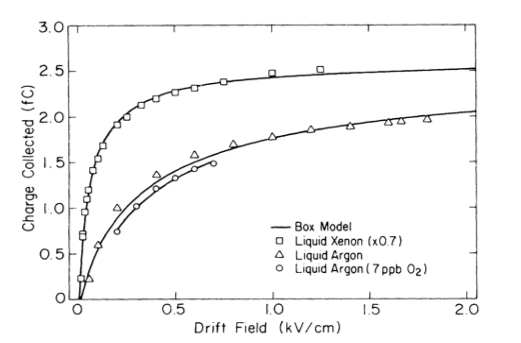
\includegraphics[width=0.8\textwidth]{TIRecombination}
\caption{Measurements of charge collected $q \propto 1 - r$ for LAr and LXe vs. $E$.  Squares correspond to LXe and were measured with
$\xi E = 0.15\ \mathrm{kV\ cm^{-1}}$.  Triangles and circles are LAr and were measured at $\xi E = 0.84\ \mathrm{kV\ cm^{-1}}$.  Curves
are best fit for box model (\citeref{Thomas1987}).}
\label{fig:ti_recomb}
\end{figure}

If an electric field is applied the \electron that have sufficiently large thermal energy are drifted for
proportional scintillation, conserving the measurable quantity.

The decrease in scintillation yield for $\beta$ and $\gamma$ is only observed at low LET where the ionization density is relatively low.  The
lack of neighboring $\mathrm{Xe}^{+}$ limits the probability of recombination with a non-parent ion.  At higher LET the ion density
is sufficient for essentially 100\% recombination and results in a flat top region as seen in \figref{fig:scintillation_yield}.  This
effect is not technically quenching because there is no true decrease in photons and electrons.

\begin{figure}
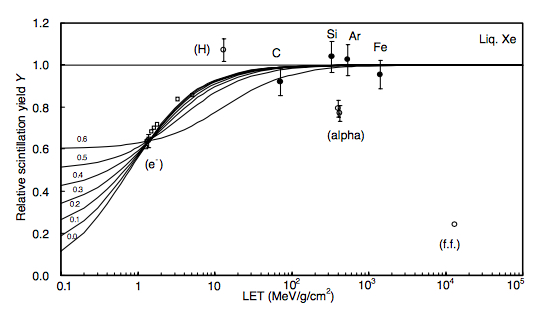
\includegraphics[width=0.8\textwidth]{ScintillationYield}
\caption{Scintillation yield as a function of LET in LXe.  Open circle represent electrons, alpha particles, and fission fragments.  Solid
circles represent relativistic heavy particles.  Open squares represent gamma-ray.  Solid lines represent various fits to the
$\beta$-$\gamma$
data performed in \citeref{Doke2002} and are not discussed here.  Image credit: \citeref{Doke2002}.}
\label{fig:scintillation_yield}
\end{figure}

\begin{figure}
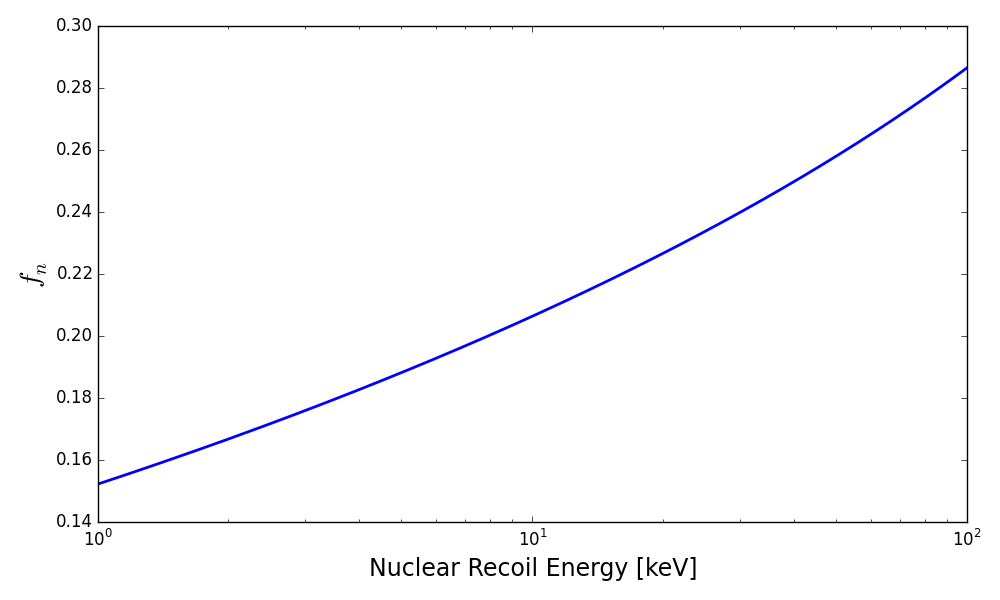
\includegraphics[width=0.8\textwidth]{Lindhard}
\caption{Fraction of nuclear energy passed to atomic motion in xenon using Lindhard's theory (\citeref{Lindhard1965}).}
\label{fig:lindhard}
\end{figure}

In an electric field $E$ an \electron that is freed but does not recombine with its parent or other ionized atoms will move anti-parallel
to the field at drift velocity $v_{d}$.  For $E \lesssim 100\ \mathrm{V\ cm^{-1}}$ \vd$\propto E$, $100 \lesssim E \lesssim 10^{3-4}$
\vd$\propto E^{1/2}$, and $E \gtrsim 10^{4}$ \vd plateaus at $\sim 3\ \mathrm{mm\ \mu s^{-1}}$ (\citeref{Miller1968}).

\begin{table}
 \centering
 \begin{tabular}{cc}
 \hline
 $E$ [V cm$^{-1}$] & \vd [mm $\mu$s$^{-1}$] \\
 \hline
 $\lesssim 100$ & \vd$\propto E$ \\
 $\sim 100-10^{3-4}$ & \vd$\propto E^{1/2}$ \\
 $\gtrsim 10^{4}$ & \vd$\sim 3$ \\
 \hline
 \caption{Drift velocity \vd as a function of electric field $E$ for LXe}
 \end{tabular}
\end{table}

\begin{figure}
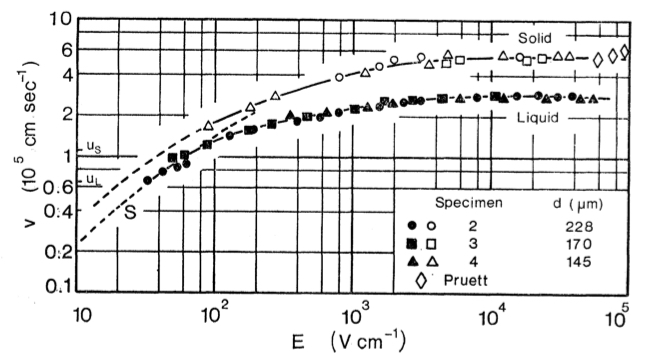
\includegraphics[angle=0.5, width=0.8\textwidth]{DriftVelocity}
\caption{Drift velocity for solid and liquid xenon}
\label{fig:drift_velocity}
\end{figure}

As the electron cloud drifts it will diffuse both longitudinally (in the direction of $E$) and transversely (perpendicular to $E$).  The
diffusion coefficients $D_{L}$ and $D_{T}$ are dependent on the electric field with $D_{T}/D_{L} \sim 10$.  The electron spread can
be written as $\sigma_{D_{T}} = \sqrt{D_{T} t_{d}}$ where $t_{d} = d/$\vd is the drift time and $d$ is the drift distance.

Extensive xenon distillation and purification occurs before it is used in a detector.  Nonetheless impurities outgas from detector
material and contaminate the LXe.  Electronegative impurities in particular present a problem since they will attach to a free \electron,
lowering the number that reach the top of the detector and decreasing the secondary scintillation as shown in \eqref{eq:imp_attach}.

\begin{equation}
e^{-} + S \rightarrow S^{-}
\label{eq:imp_attach}
\end{equation}

\noindent The amount of \electron captured is dependent on the time in the LXe.  Thus an advantage of larger \efields is a larger
\vd (up to a point) and thus less time in the liquid.  Doping LXe with organic materials such as butane can increase \vd at higher
\efields but they are not used in DM detectors due to difficulty in purifying (\citeref{Yoshino1976}).  By setting the rate at which
electrons are absorbed by impurities $dq/dt = -qk_{S}S$ where $S$ is the impurity concentration and $k_{S}$ is the attachment rate
constant we find

\begin{equation}
q(t) = q_{0}e^{-tk_{S}S} = q_{0}e^{-t/\tau_{e}}
\label{eq:lifetime_equation}
\end{equation}

\noindent where $\tau_{e} = (k_{S}S)^{-1}$ and is known as the electron lifetime.  $k_{S}$ is shown in \figref{fig:attachment_rate} for
O$_{2}$,
N$_{2}$O, and SF$_{6}$.  We see that for N$_{2}$O the attaching rate constant increases with \efield whereas \otwo and SF$_{6}$
decerase.  Typically impurity concentration is given in O$_{2}$-equivalent values - that is, the concentration of \otwo if it was solely
responsible for \electron attachment.  For modeling electron lifetime it turns out that using the \otwo curve in
\figref{fig:attachment_rate} gives a good approximation.  Removing such impurities will be discussed in detail in \secref{}.


\begin{figure}
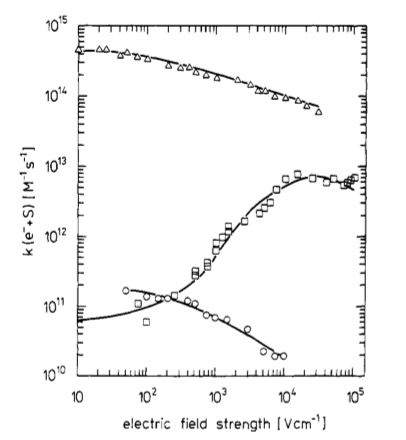
\includegraphics[width=0.8\textwidth]{AttachmentRate}
\caption{Attaching rate constant $k_{S}$ from \citeref{Bakale1976} for \otwo, N$_{2}$O, and SF$_{6}$ with respect to electric field.  At
larger \efield $k_{S}$ increases for N$_{2}$O and decreases for \otwo and SF$_{6}$.}
\label{fig:attachment_rate}
\end{figure}

In a TPC a cathode at the bottom of the detector applies an electric field in the LXe.  The \electron drift towards the top where a
grounded gate rests a few millimeters below the LXe surface.  Directly above the gate by a couple centimeters is the anode, which
applies a strong electric field that extracts the electrons into the gas xenon (GXe).  An extracted electron will ionize and excite
GXe atoms, whose freed electrons will do so as well in what is known as electroluminescence.  The number of ionized and excited atoms
is proportional to the number of \electron extracted, hence it is also known as proportional scintillation.  The number of photons
$N_{\mathrm{ph}}$ produced traveling a distance $z$ is

\begin{equation}
\frac{dN_{\mathrm{ph}}}{dz} = \alpha \Big( \frac{E_{g}}{P} - \beta \Big) P
\label{eq:electronlum}
\end{equation}

\noindent where $\alpha = 70\ \mathrm{photons\ kV^{-1}}$, $\beta = 1.0\ \mathrm{kV\ cm^{-1}\ atm^{-1}}$, and $E_{g}$ and $P$ are the
GXe electric field and pressure, respectively (\citeref{Belogurov1995}).



%====================================
\section{Stopping Power}
\label{sec:stopping_power}
A particle that produces an electronic recoil will lose energy through inelastic collisions with electrons, prompting ionization or
excited states.  The energy lost per unit
length is the electronic stopping power and denoted $dE/dx$, which is related to the linear energy transfer (LET).  It depends on the
type and energy of the particle and properties of the
medium including density and composition.  A larger electronic stopping power indicates the particle will slow more quickly, thereby
depositing its energy densely along its trajectory.  This is known as self-shielding, and is an
important characteristic of a detector.  A larger self-shielding will restrain external radiation from penetrating deep in the detector,
which allows a larger fiducial volume (FV) for dark matter detection.  Because the stopping power is proportional to the
density of the medium, LXe is more effective at self-shielding than liquid argon ($1.395\ \mathrm{g\ cm^{-3}}$) and liquid neon
($1.207\ \mathrm{g\ cm^{-3}}$).

By dividing the stopping power by the medium's density we get a function that is mainly a function of the radiating particle known as
the mass stopping power.  This is shown for $\alpha$, $e^{-}$, and protons in \figref{fig:mass_stopping_power}.  We see that for the DM
region of interest ($1-100$ keV) as \electron
energy increases the stopping power decreases, while for $\alpha$ and protons the reverse is true.  Multiplying by the density of LXe
$\rho_{\mathrm{LXe}}$ gives an electron stopping power of $0.65-30\ \mathrm{keV\ \mu m^{-1}}$ for \electron and
$\sim 20-900\ \mathrm{keV\ \mu m^{-1}}$ for $\alpha$ and protons.

We can see that in
the dark matter search region ($1-100$ keV) $e^{-}$ decrease by a factor of $\sim 10$.  Multiplying by the density of LXe we get the
electronic stopping power to be $\sim 0.65-30\ \mathrm{keV\ \mu m^{-1}}$.  \alphadecays are typically $> 5.5$ MeV and thus have a stopping
power of $\sim 600-2000\ \mathrm{keV\ \mu m^{-1}}$.  We see that particle tracks are on the order of $10 \mathrm{\mu m}$, so particles that
originate at or outside the surface of the detector will never make it into the FV with any reasonable probability.

\begin{figure}[t]
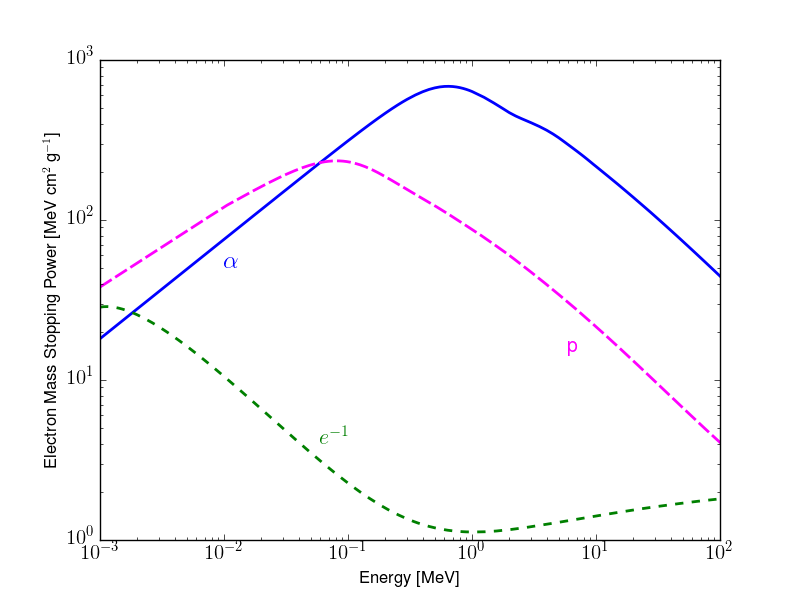
\includegraphics[width=0.8\textwidth]{MassStoppingPower}
\caption{Electron mass stopping power for $\alpha$, $e^{-}$, and protons.  (\citeref{Berger2018a})}
\label{fig:mass_stopping_power}
\end{figure}[t]

Since a higher stopping power translates to a larger decrease in energy, there will be a higher ionization density in the particle
track.  This has implications that will be discussed in \secref{}.

For particles that induce a nuclear recoil we must also consider the nuclear stopping power, which is the energy lost per unit length from
atomic collisions that transfer kinetic energy to the nucleus.  Thus for NR the total stopping power is

\begin{equation}
\bigg( \frac{dE}{dx} \bigg)_{\mathrm{tot}} = \bigg( \frac{dE}{dx} \bigg)_{\mathrm{elec}} + \bigg( \frac{dE}{dx} \bigg)_{\mathrm{nuc}}
\end{equation}

\noindent Atomic motion in liquid noble gas experiments is not observable so the number of quanta $N_{q}$ produced will be lower
than for an an electronic recoil scatter with the same recoil energy.  While energized electrons are capable of transferring very small
amounts of energy to the motion of the nucleus, the reverse is not true.  Thus all translational energy acquired by the nucleus is
resigned to be unobservable.  The fraction of energy lost to atomic motion is characterized by $f_{n}$.

Moreover, energized electrons can transfer a very small amount
of energy to the motion of the atom, but
the reverse is not true.  The fraction of energy lost to atomic motion $f_{n}$ is commonly characterized with the Lindhard model
(\citeref{Lindhard1965})

\begin{equation}
f_{n} = \frac{k g(\epsilon)}{1 + k g(\epsilon)}
\label{eq:linhard_quenching}
\end{equation}

\noindent where $k = 0.133Z^{2/3}A^{1/2}$, $g(\epsilon) = 3\epsilon^{0.15} + 0.7\epsilon^{0.6} + \epsilon$, and
$\epsilon = 11.5 (E_{R} / Z^{7/3})$ where $Z$ is the atomic number and $A$ is the number of nucleons.  $k$ is proportional to the ratio of
electronic stopping power to particle velocity of the recoiling Xe atom (\citeref{Sorensen2011}) and $g(\epsilon)$ is proportional
to the ratio of electronic to nuclear scaling factor (\citeref{NEST2015}).  There has been some debate about
the coefficient in $k$ and I use the value from \citeref{Lewin1996}.  Studies have shown that energy is only lost to atomic motion for
nuclear recoils.  The quenching factor $f_{n}$ is shown in \figref{fig:lindhard} for the relevant energy search region.


%====================================
\section{Interactions}
\label{sec:interactions}
Because WIMP searches usually expect an interaction with an atom's nucleus, electronic recoils are not investigated for possible
signal.  Instead they play two major roles - the first is for calibrating the detector.  For larger detectors external sources are
not efficient since the the self-shielding of Xe makes it nearly impossible for radiation to penetrate the interior.  Thus internal
sources with short half-lifes such as \kryptonmeta and \radoncal are used.  The second role ER play is background to the DM
search.  Detector materials have radioactive elements that decay inside the detector, and long-lived intrinsic sources such as
the inevitable residual \krypton and \radon that passed the Xe distillation process.  The latter is much more concerning as events from
detectors materials cannot breach the fiducial volume, but intrinsic sources are uniformly distributed and must be understood.

\subsection{Photons}
\label{subsec:photons}
Photons produce electron recoils as they interact with \electron via Compton scattering pair production, or photoelectric absorption
as shown in \figref{fig:phot_atten}.  In Compton scattering the photon
recoils off of an \electron, transferring a portion of its energy.  Nuclear Compton scattering is possible but much rarer.  If the
angle of the scatter is known the change in energy can be determined.

Pair production is when a high-energy photon produces a particle-antiparticle pair.  Typically this refers to a photon passing sufficiently
near to an atom's nucleus creating an electron-positon pair.  The proximity of the nucleus is required to conserve momentum so it
recoils slightly as well.  The photon must have an energy of at least twice the mass of the electron $m_{e}$, or 1.022 MeV.  Pair production
also occurs for a photon in the presence of an atomic electron but is less probable and requires an energy of at least $4m_{e}$.  This
is known as triplet production since the recoiling electron will create a track in addition to the electron-positon pair
(\citeref{Hubbell2006}).  At high energies pair production becomes the dominant interaction for photons and matter.

Photoelectric absorption is when an electron absorbs the energy of the photon and is freed from its electron shell.  In this case the
photon disappears entirely and the kinetic energy of the electron is equal to the photon's energy minus the electron binding energy.  This
is a useful tool for calibrating small detectors with mono-energetic \gammarays from elements such as \cesium (661.7 keV) and \cobaltsixty
(1.1732 and 1.3325 MeV).  For larger detectors however the self-shielding prevents even the higher \gammarays from reaching the fiducial
volume, so external sources cannot be used for calibration.  Photoelectric absorption is the dominant interaction in the WIMP detection
energy region of interest, as shown in \figref{fig:phot_atten}.

\begin{figure}
 \centering
 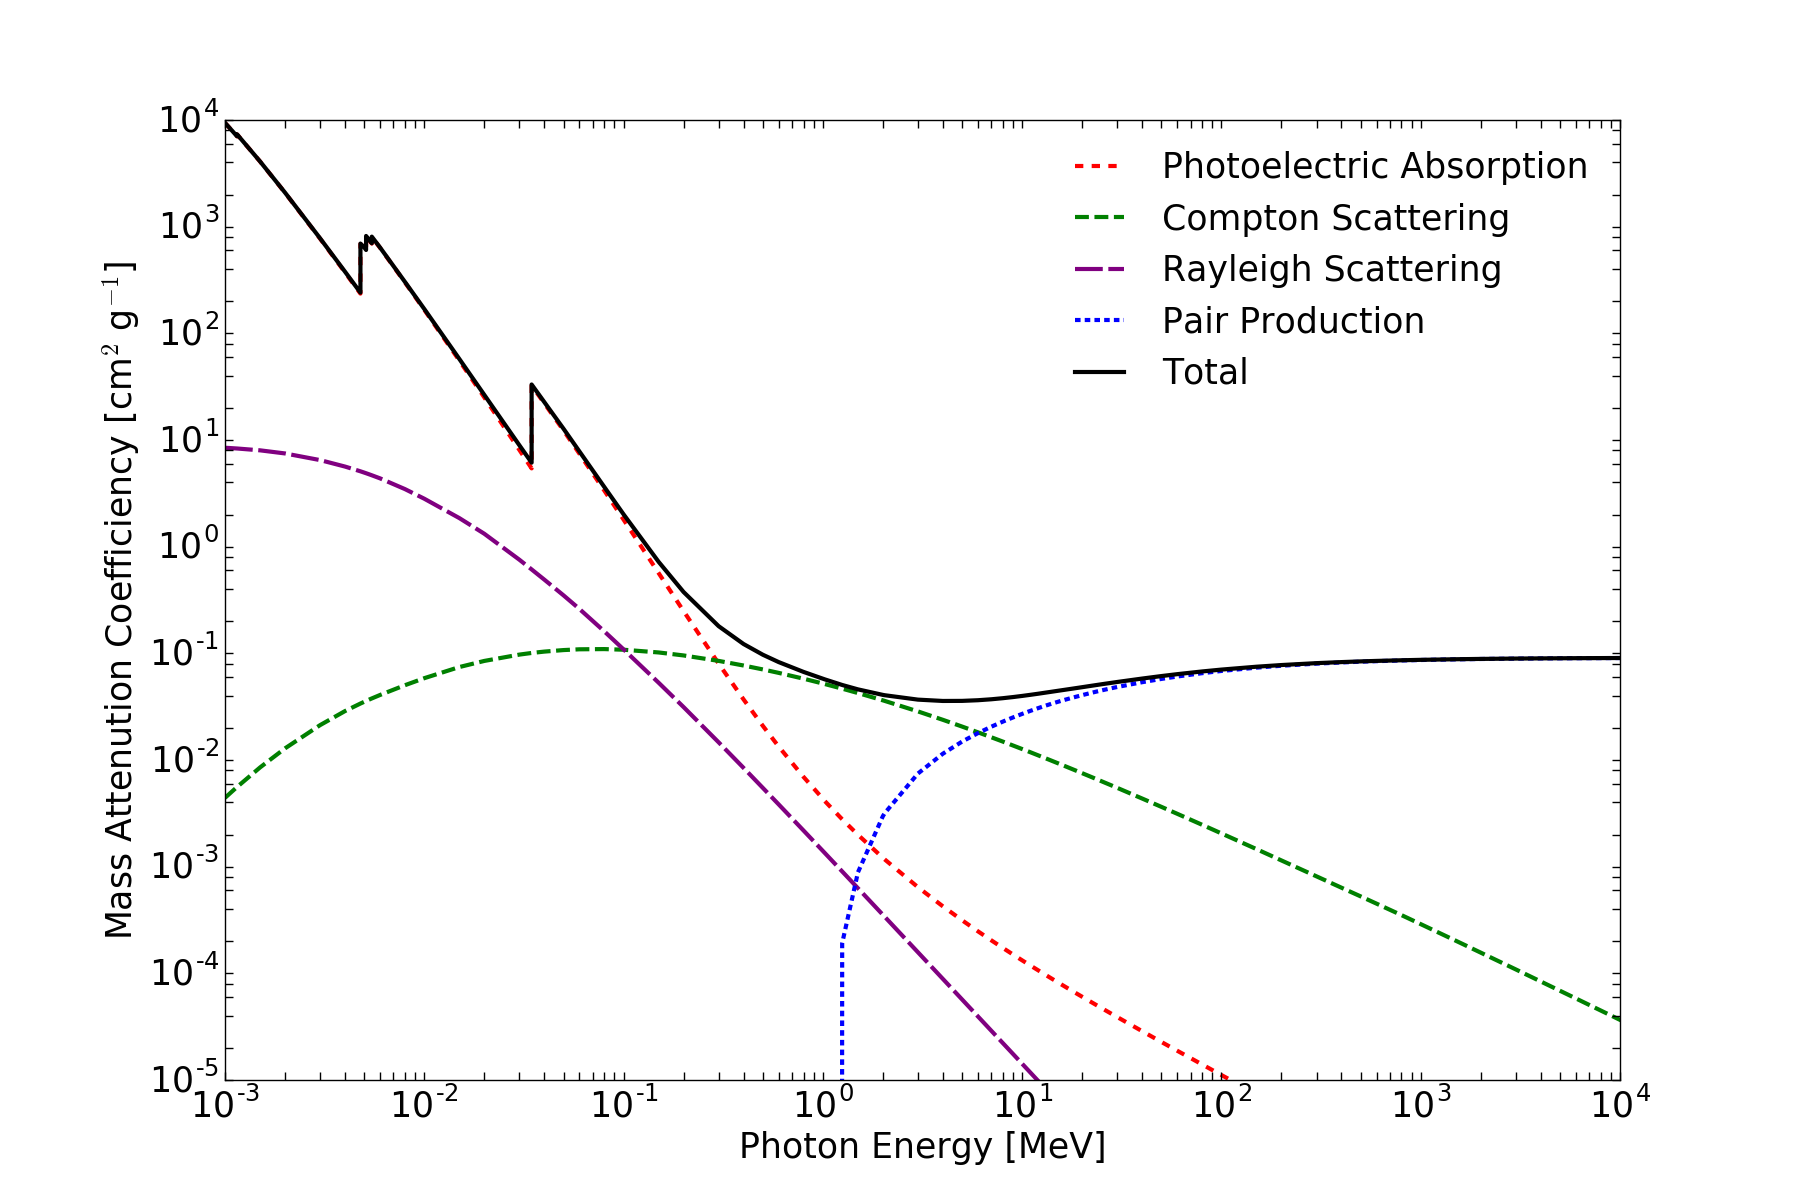
\includegraphics[width=0.8\textwidth]{PhotonAttenuation}
 \caption{Mass attenuation coefficient for photon energies $10^{-3} - 10^{4} \mathrm{MeV}$.  In addition to the total, values for
 photoelectric absorption,
 Compton scattering, and pair production are shown}
 \label{fig:phot_atten}
\end{figure}


\subsection{$\beta$-Decays}
\label{subsec:beta}
\betadecays are the emission of an electron-antineutrino (positron-neutrino) from a neutron (proton).  As with photons, they interact
with the \electron shell and thereby produce electronic recoils.  Because the neutrino carries
some momentum, the energy spectrum of the \electron is not mono-energetic, which makes it harder to identify the origin.  In Xe
experiments \betadecays contribute the most contamination in the search region for this reason and that they occur roughly uniformly
throughout the detector.  \krypton decays via

\begin{equation}
\ce{^{85}Kr} \rightarrow \ce{^{85}Rb} + e^{-} + \overline{\nu_{e}}
\end{equation}

\noindent with an energy of 687 keV with 99.53\% and 173 keV followed by a 514 $\gamma$ with 0.47\%.  These low-energy \betadecays
contaminate the search region, and a half-life of 10.72 years ensures \krypton will be present throughout the lifetime of the
experiment.

\radon presents a similar problem.  As a daughter of the \uranium decay chain it emanates from the detector materials and distributes
uniformly throughout the detector.  Its two most dangerous daughters or \leadtwofourteen and \bismuthtwofourteen, each of which
undergo \betadecay.  \bismuthtwofourteen is easily identifiable because its daughter \poloniumtwofourteen has a half-life of
$160\ \mathrm{\mu s}$ and undergoes \alphadecay.  Thus a cut on coincidence can remove such events.  \leadtwofourteen is more
dangerous, as it has no coincidence cut with its parent or daughter.  Its end-point energy when it decays to the ground state of
\bismuthtwofourteen is 1019 keV, which contaminates the region of interest.  More concerning is a decay to higher energy levels, which
if near the border of the fiducial volume has a risk of the subsequent \gammaray exiting undetected.  In XENON100 recoiling daughters of
the \radon decay chain were observed to drift towards the cathode, possibly the result of becoming positively ionized
(\citeref{Weber2013}), lowering the number of \betadecays in the region of interest.


\subsection{Neutrinos}
\label{subsec:neutrinos}
Neutrinos impact both electronic and nuclear recoil spectra at low energies.  Solar neutrinos can elastically scatter off \electron
producing an ER.  \textit{pp} neutrinos make up 92\% of these scatters, with \ce{^{7}Be} making 7\%, and all other sources contributing
$<1$\% (\citeref{Aprile2016}).

Coherent neutrino-nucleus scattering produces nuclear recoils.  The majority of the interactions in the ROI come from Solar \ce{^{8}Be}
and \textit{hep} neutrinos, as those at higher energy from sources such as diffuse supernovae and the atmosphere have a significantly
lower rate.

Neutrinos are an irreducible background that affects our detector uniformly.


\subsection{Neutrons}
\label{subsec:neutrons}
Neutrons in our detector come from two main sources: the spontaneous fission (mainly $\alpha$) of isotopes of primordial chains of
\uranium, \ce{^{235}U}, and \ce{^{232}Th} from detector materials (radiogenic neutrons), and muons
passing through the rock and material above and around the detector (cosmogenic neutrons).  The former has energies in the MeV range
while the latter can reach tens of GeV (\citeref{Aprile2016}).  Neutrons have a mean free path on the order of tens of cm, which makes
them more difficult to shield than $\alpha$, $\beta$, or $\gamma$ scatters.  Furthermore, neutrons can produce nuclear recoils, making
them indistinguishable from WIMPs.  It is critical then to have a thorough understanding of the neutron background so a reliable
estimate of the number of events in the signal region to avoid mistaking a neutron as a WIMP or vice versa.

Neutrons will scatter elastically, inelastically, or be radiatively absorbed by the Xe nucleus.  Radiative absorption is when the
Xe nucleus captures the neutron, extending its atomic mass by one.  Fortunately, such an increase typically leads to another stable
xenon atom.  Exceptions are \ce{^{125}Xe}, \ce{^{127}Xe}, \ce{^{133}Xe}, and \ce{^{135}Xe}, which are listed in \tabref{tab:ncaption_xe}
along with subsequent decays and half-lives.  \ce{^{125}I} and \ce{^{135}Cs} have sufficiently long half-lives that they will be removed
by the getters from the LXe before they decay along with stable daughters \ce{^{127}I} and \ce{^{133}Cs}.

\bgroup
\def\arraystretch{1.4}
\begin{table}
 \centering
 \begin{tabular}{cccc}
 \centering
 Isotope & Decay & Energy [keV] & Half-Life \\
 \hline
 \ce{^{125}Xe} & $\ce{^{125}Xe} \rightarrow \ce{^{125}I} + \beta^{+} + \nu_{e}$ & 622.17 & 16.89 h \\
  & $\ce{^{125}I} + e^{-} \rightarrow \ce{^{125}Te} + \nu_{e}$ & 185.77 & 59.38 d \\
 \ce{^{127}Xe} & $\ce{^{127}Xe} + e^{-} \rightarrow \ce{^{127}I} + \nu_{e}$ & 662.33 & 36.34 d \\
 \ce{^{133}Xe} & $\ce{^{133}Xe} \rightarrow \ce{^{133}Cs} + \beta^{-} + \overline{\nu_{e}}$ & 427.36 & 5.24 d \\
 \ce{^{135}Xe} & $\ce{^{135}Xe} \rightarrow \ce{^{135}Cs} + \beta^{-} + \overline{\nu_{e}}$ & 1164.8 & 9.14 h \\
  & $\ce{^{135}Cs} \rightarrow \ce{^{135}Ba} + \beta^{-} + \overline{\nu_{e}}$ & 268.66 & $2.315 \times 10^{6}\ \mathrm{y}$ \\
 \hline
 \end{tabular}
 \caption{Radioactive isotopes of Xe produced from neutron capture.  Decays are shown to stable elements along with decay energies and
 half-lives}
 \label{tab:ncaption_xe}
\end{table}
\egroup

Inelastic scattering involves the neutron exciting the Xe nucleus.  It will still recoil from a nuclear interaction, but the Xe
activation follows with emission of a $\gamma$-ray.  The most relevant isotopes for our detector are \ce{^{129}Xe} and \ce{^{131}Xe},
which have half-lives of 0.97 and 0.48 ns and decay with energies 36.9 and 80.2 keV, respectively.  These lifetimes are so short that
they will most likely be merged with the energy deposit of the nuclear recoil.  Additionally longer-lived activations for metastable
states \ce{^{129m}Xe} and \ce{^{131m}Xe} that decay with with half-lives 8.88 and 11.93 days and energies 236.14 and 163.93 keV.  The
longer lifetimes allow the metastable xenon to become distributed uniformly throughout the detector, providing an internal calibration
over a period of weeks, which can be taken during dark matter data taking.

\begin{figure}
\includegraphics[\width=0.8\textwidth]{Fig. 2 from https://arxiv.org/pdf/1512.00460.pdf}
\label{fig:nr_elastic_inelastic}
\end{figure}
The final interaction type is elastic scattering.  In this scenario the neutron rebounds from the nucleus and kinetic energy after the
scatter is preserved and distributed between the neutron and recoiling Xe atom.  This is discussed further in \secref{sec:nr} and
\chapref{}.

https://arxiv.org/pdf/1512.00460.pdf

%====================================
\section{Electronic Recoils}
\label{sec:er}
An electronic recoil signifies that the interaction occurred with the electron shell of an atom and the particle.  Because no energy
is lost to atomic motion the number of quanta produced is \nquant$ = $\energyer$ / W$ where \energyer is the electronic recoil energy
and $W = 13.2\ \mathrm{eV}$ (\citeref{Dahl2009}) is the energy needed to produce a single quanta.  This can be broken up into

\begin{equation}
N_{q} = N_{\mathrm{ex}} + N_{\mathrm{i}}
\label{eq:quanta}
\end{equation}

\noindent where \nex and \nion is the number of excitons and ions, respectively.  Rearranging we can find the probability that a
given quanta is an ion

\begin{equation}
p_{\mathrm{ion}} = \frac{1}{1 + \frac{ N_{\mathrm{ex}} }{ N_{\mathrm{ion}} }}
\end{equation}

\noindent with $p_{\mathrm{ex}} = 1 - p_{\mathrm{ion}}$.  The ratio $N_{\mathrm{ex}} / N_{\mathrm{ion}}$ has been calculated to be
0.06 (\citeref{Takahashi1975})
but measurements disagree (\citeref{Doke2002, Aprile2007}).  Currently $N_{\mathrm{ex}} / N_{\mathrm{ion}}$ is taken to be between
0.13-0.2.  The number of
photons and electrons after recombination can be found as

\begin{equation}
N_{\mathrm{phot}} = N_{\mathrm{ex}} + rN_{\mathrm{i}} \\
N_{\mathrm{e}} = (1 - r)N_{\mathrm{i}}
\end{equation}

\noindent where \nphot is the number of photons produced and \nelect is the number of \electron that do not recombine and are extracted as
proportional scintillation.

Although noble gas detectors allow ER-NR discrimination, the two regions are near one another and have overlap where an event could
be considered with reasonable probability to be either.  In the DM search only the region of NR-space where the NR likelihood is
significantly more probable is used.  To minimize the risk of ER, or background events from occurring in the signal region it is
critical to reduce the background as much as possible, and with the ton-scale era of DM detectors underway much effort is being put into
material screening and enhanced xenon distillation.


%====================================
\section{Nuclear Recoils}
\label{sec:nr}
Although the vast majority of background comes from electronic recoils, nuclear recoils are more dangerous because they replicate
WIMP interactions.  Therefore the NR background must be well-modeled to avoid mistaking a background event for a WIMP or vice
versa.

Because some energy in nuclear recoils goes into atomic motion the number of excitons and ions is reduced compared to ERs.  The toal
number of quanta is $N_{q} = L E_{R} / W$ where $L$ is the Linhard quenching factor defined in \eqref{eq:linhard_quenching}.








In addition to improving the likelihood of spin-independent DM-nucleon scattering (\eqnref{eq:dr_de_final}), the average molar mass
$A = 131.293\ \mathrm{g\ mol^{-1}}$ provides much better stopping power than its noble gas counterparts.  The stopping power $dE/dx$
is the amount of energy lost per distance, and at low energies can be broken down into electronic and nuclear stopping power.

The electronic stopping power is the energy lost due to electronic excitations as a particle travels through the detector.  



% for stopping power look at A Model of Nuclear Recoil Scintillation Efficiency in Noble Liquids
%D.-M. Mei a,∗ Z.-B. Yin a,b,1, L.C. Stonehill c, A. Hime c


%Lewin and Smith (1996) - Lindhard factor
%Doke et al., 2002 - LET
%Miller et al., 1968 - drift velocity






%====================================
\section{Particle Interactions}
\label{sec:particles}



% for kr/xe level
%E Aprile, J Aalbers, F Agostini, M Alfonsi, F. Amaro, M Anthony, F Arneodo, P Barrow, L Baudis, B. Bauermeister, et al., “Removing krypton from xenon by cryogenic distillation to the ppq level,” The European Physical Journal C, vol. 77, no. 5, p. 275, 2017.